\chapter{LaTeX Docker \\
\small{\textit{-- Annanya Jain, Gavin Lam, Luo Xu}
\index{LaTeX Docker} 
\index{Chapter!LaTeX Docker}
\label{Chapter::LaTeX Docker}}}


In this chapter, we created a Docker container to compile a simple LaTeX document using TeX Live, which is basically what Overleaf does. \medskip

\section{Steps taken for creating the docker container to compile a LaTeX File}

I created the following files in a folder named: texlive-app:

\begin{minted}{text}
texlive-app/
├── Dockerfile
└── main
\end{minted}

\subsection{main.tex}

\begin{minted}{latex}

\begin{document}

\title{Password Policy Documentation}
\date{\today}
\maketitle
Let me take an example of LaTeX file with a simple table to compile. 
\section{Password Rules}
\begin{longtable}{|l|p{9cm}|} 
\caption{Password Rules \label{Table::Passwords}}\\
\hline
\textbf{User} & \textbf{Password Rule / Hint} \\
\hline
\endhead

devuser & At least 8 characters, include uppercase, 
lowercase, a number, and a symbol. Hint: First pet. 
\\ 
\hline

admin & Must change passwords every 90 days. Hint: Favorite City. 
\\ 
\hline

tester & Must include word banana Hint: Popular dessert item. 
\\ 
\hline

\end{longtable}

\end{document}
\end{minted}

\subsection{Dockerfile}
\begin{minted}{docker}
FROM debian:stable-slim

RUN apt-get update && apt-get install -y \
    texlive-latex-base \
    texlive-latex-recommended \
    texlive-latex-extra \
    texlive-fonts-recommended \
    texlive-fonts-extra \
    && rm -rf /var/lib/apt/lists/*

WORKDIR /data

CMD ["pdflatex", "main.tex"]
\end{minted}

\subsection{Building the Docker image}
To build and run the container:

\begin{minted}{bash}
docker build -t texlive-app .
docker run --rm -v $(pwd):/data texlive-app
\end{minted}

\begin{center}
  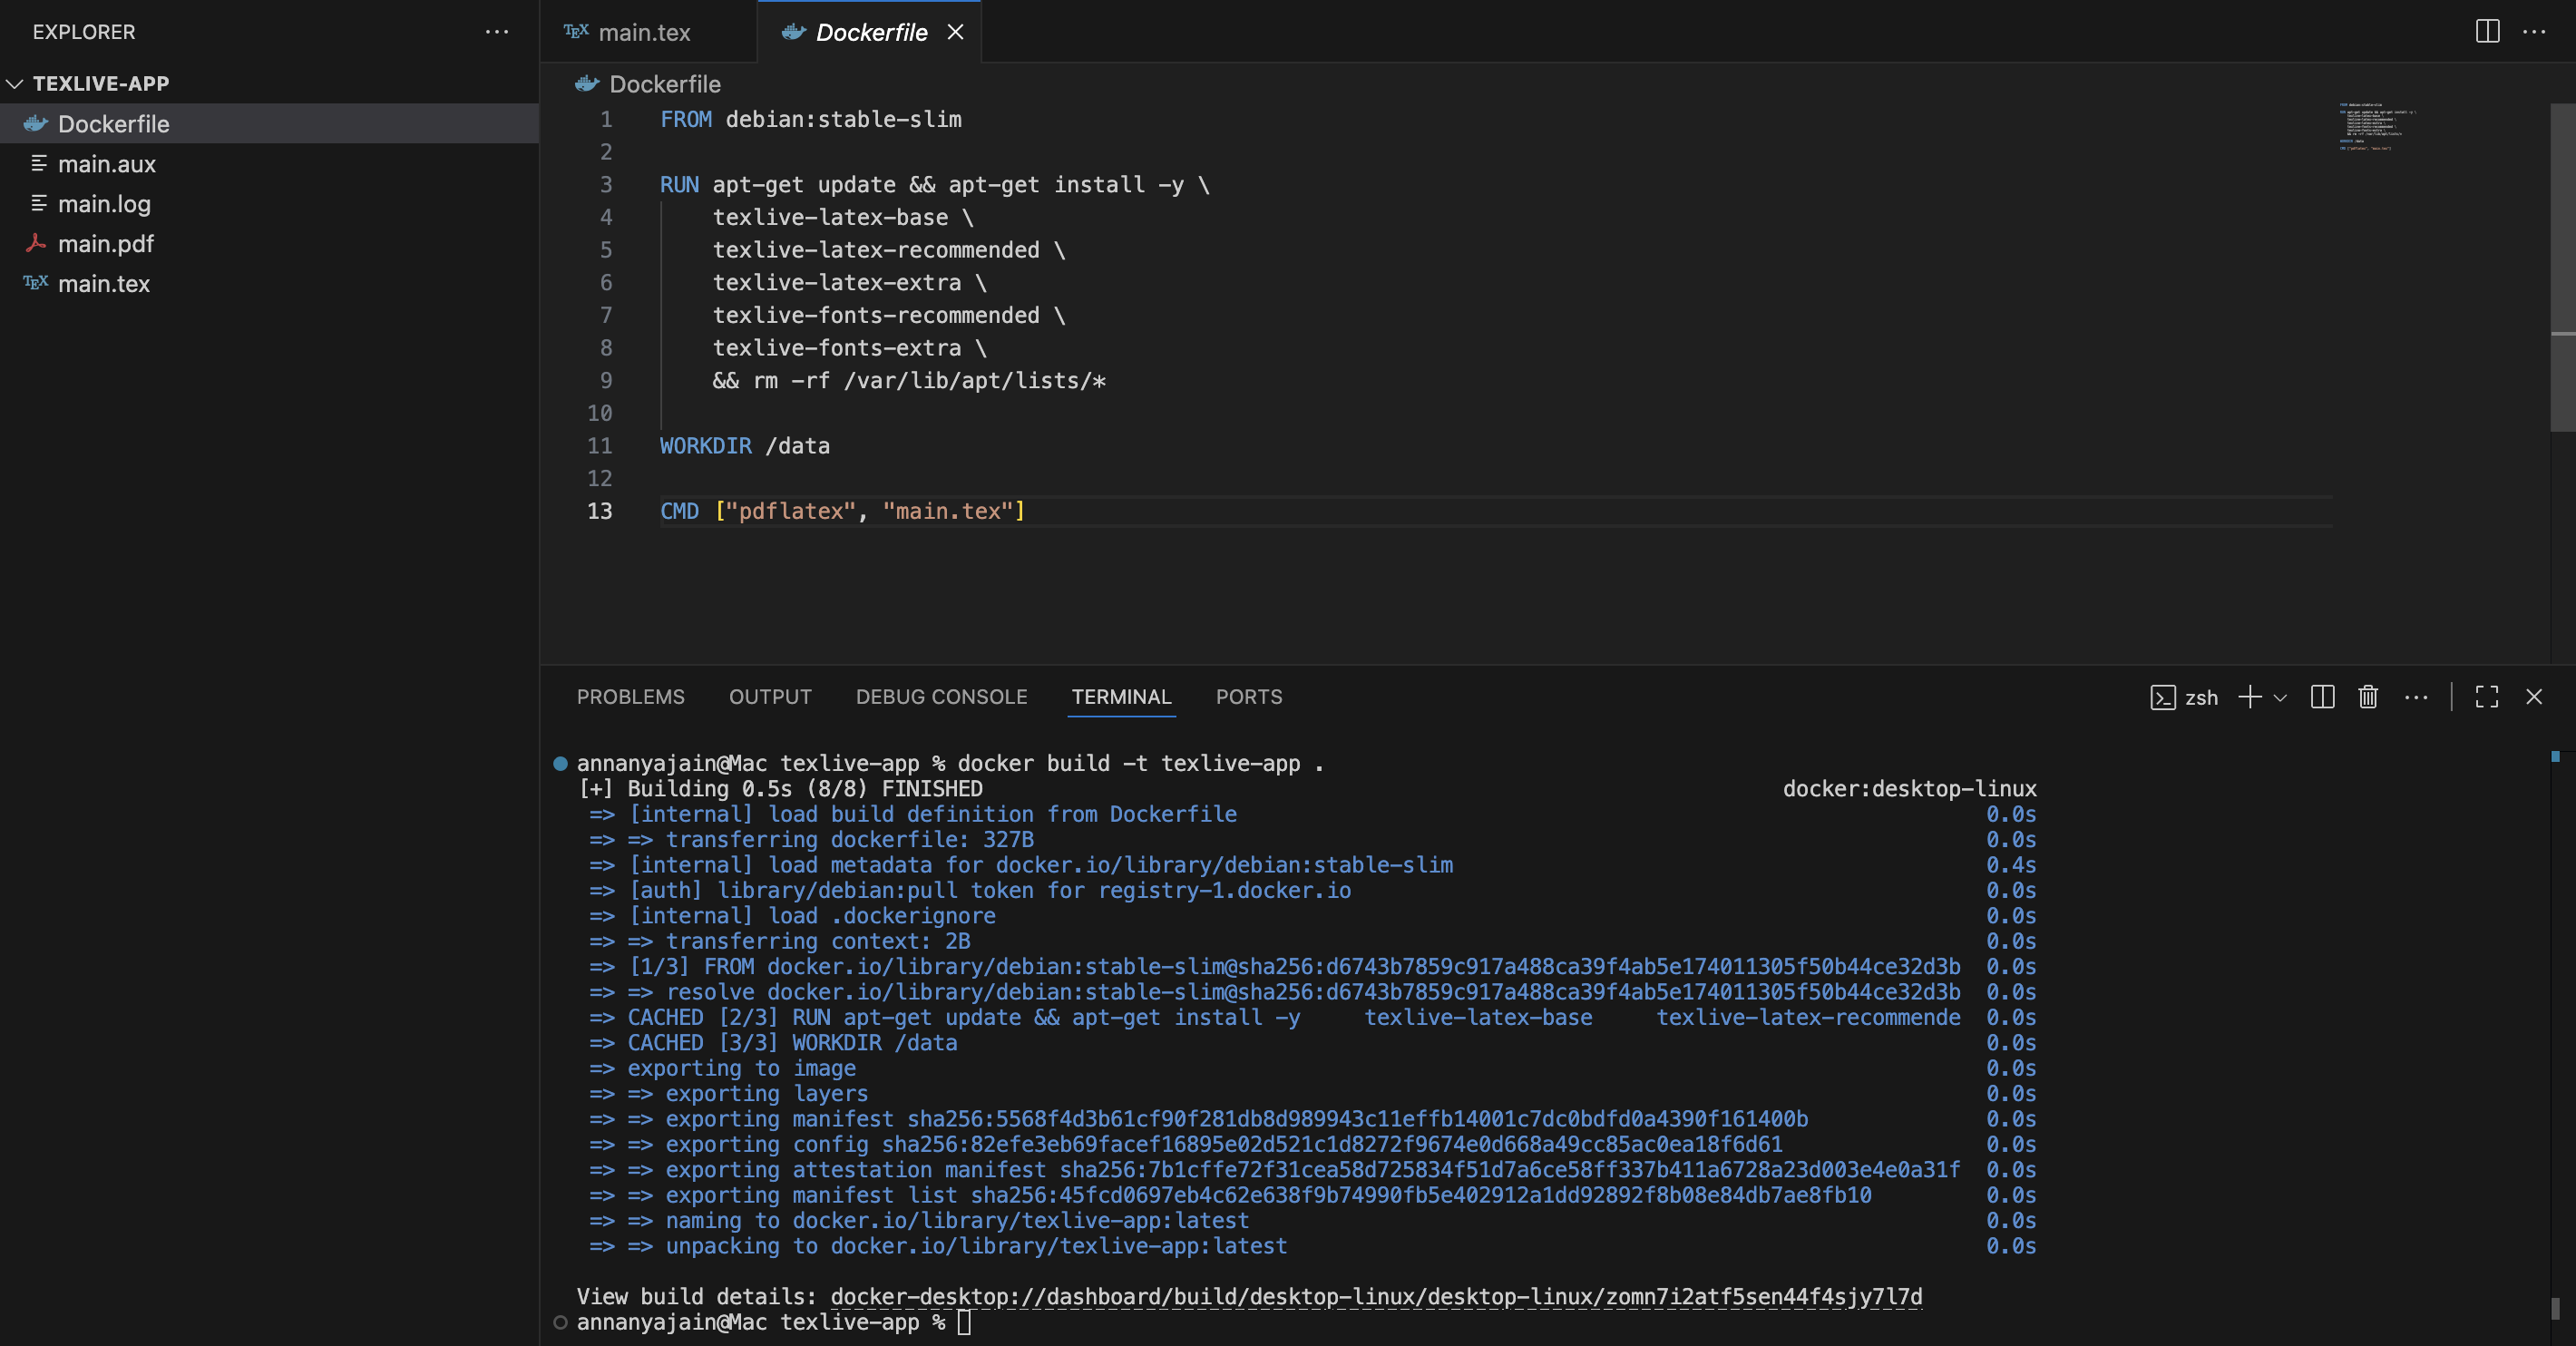
\includegraphics[width=1.0\textwidth]{png/texlive_build.png}
\end{center}

\noindent After running the commands, the output file \texttt{main.pdf} 
gets generated in the project folder on the machine. \medskip

\begin{center}
  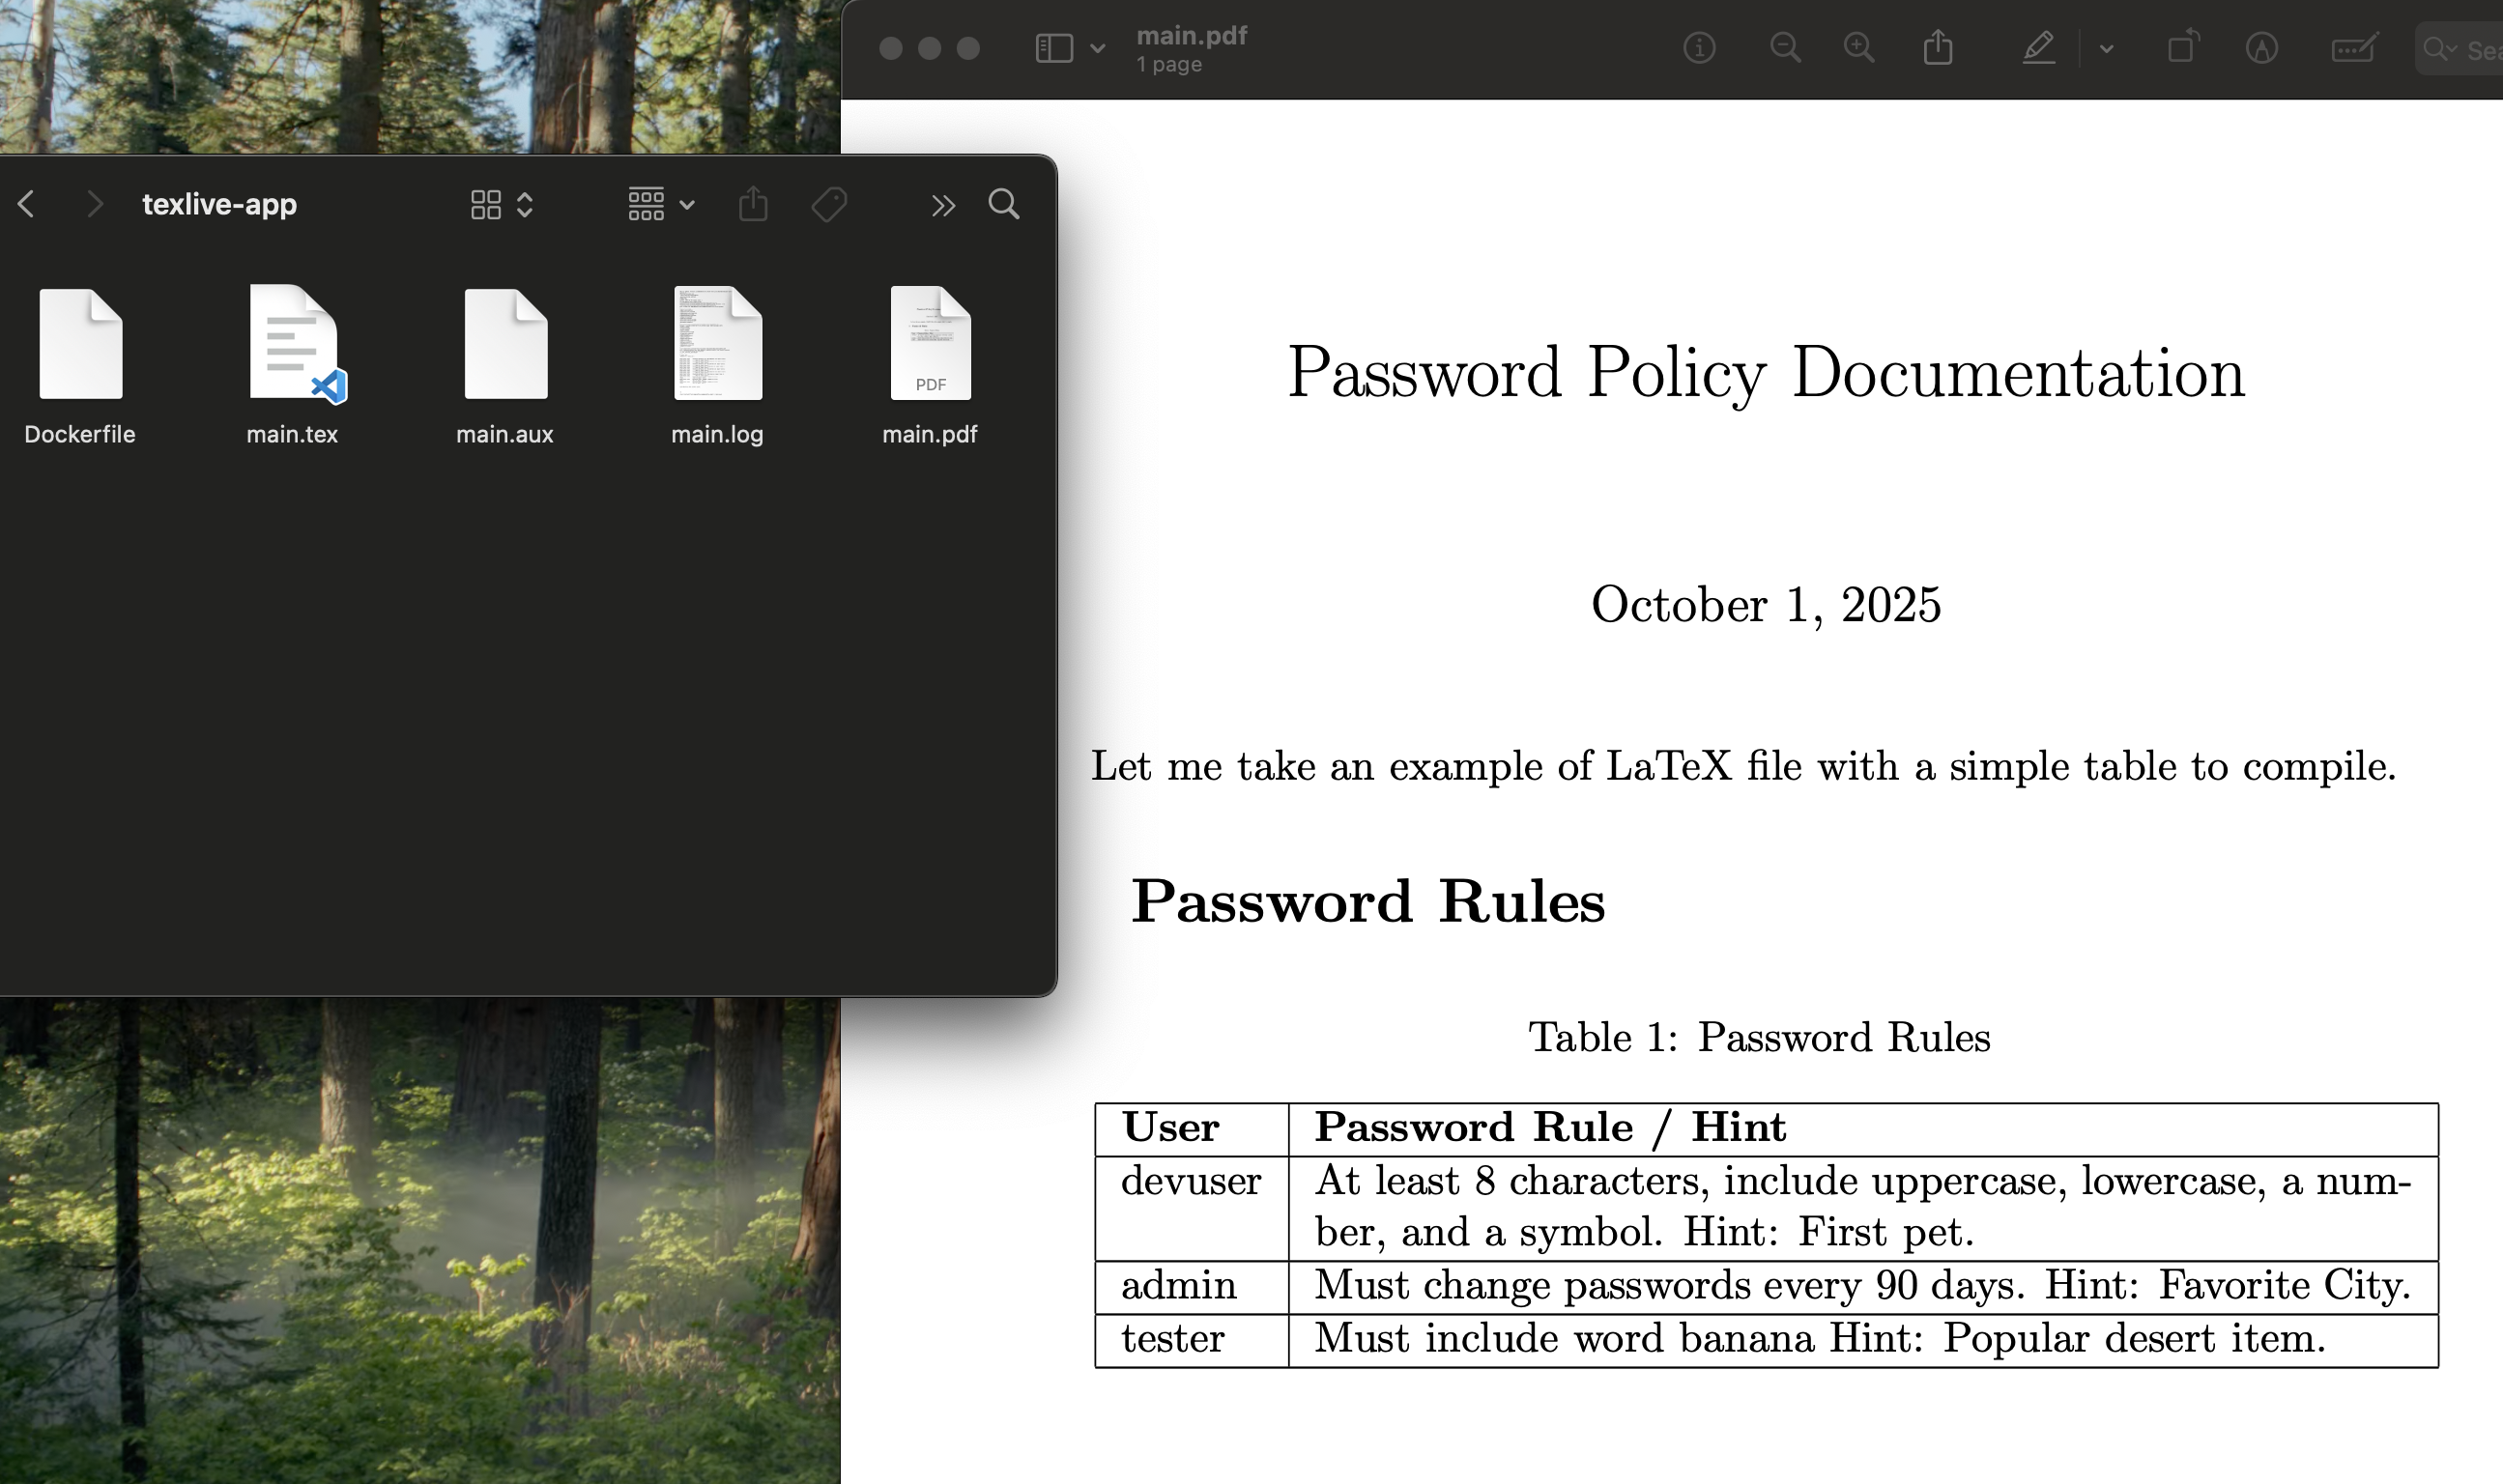
\includegraphics[width=1.0\textwidth]{png/main_pdf generated.png}
\end{center}


